% urban-short-report.tex
% v0.1 Sept. 2021

\documentclass{urban-formatting}

% Font and Font Weight
\usepackage[default]{lato}
\usepackage[T1]{fontenc}

\begin{document}
% Setting the page numbering to be roman first
\pagenumbering{roman}


%%%%%%%%%%%%%%%%%%%%%%%%%%%%%%%%%%%% Title %%%%%%%%%%%%%%%%%%%%%%%%%%%%%%%%%%%%%%

\begin{titlepage}
    % Add Policy Center/Intaitive/Toxonmy Term Bar
    % note the textbox exceeds width of document to avoid white space on sides
    \begin{textblock*}{9in}(-0.25in, 0.125in)
        \begin{tcolorbox}[valign = center]
            \begin{center}
                \policycenter{[Policy Center, Initiative, or Taxonomy Terms Here]}
            \end{center}
        \end{tcolorbox}
    \end{textblock*}

    % Adding the cover image - code forces the image to be width of full paper (ignoring margins)
    \vspace*{-1.75cm}
    \noindent
    \makebox[\textwidth]{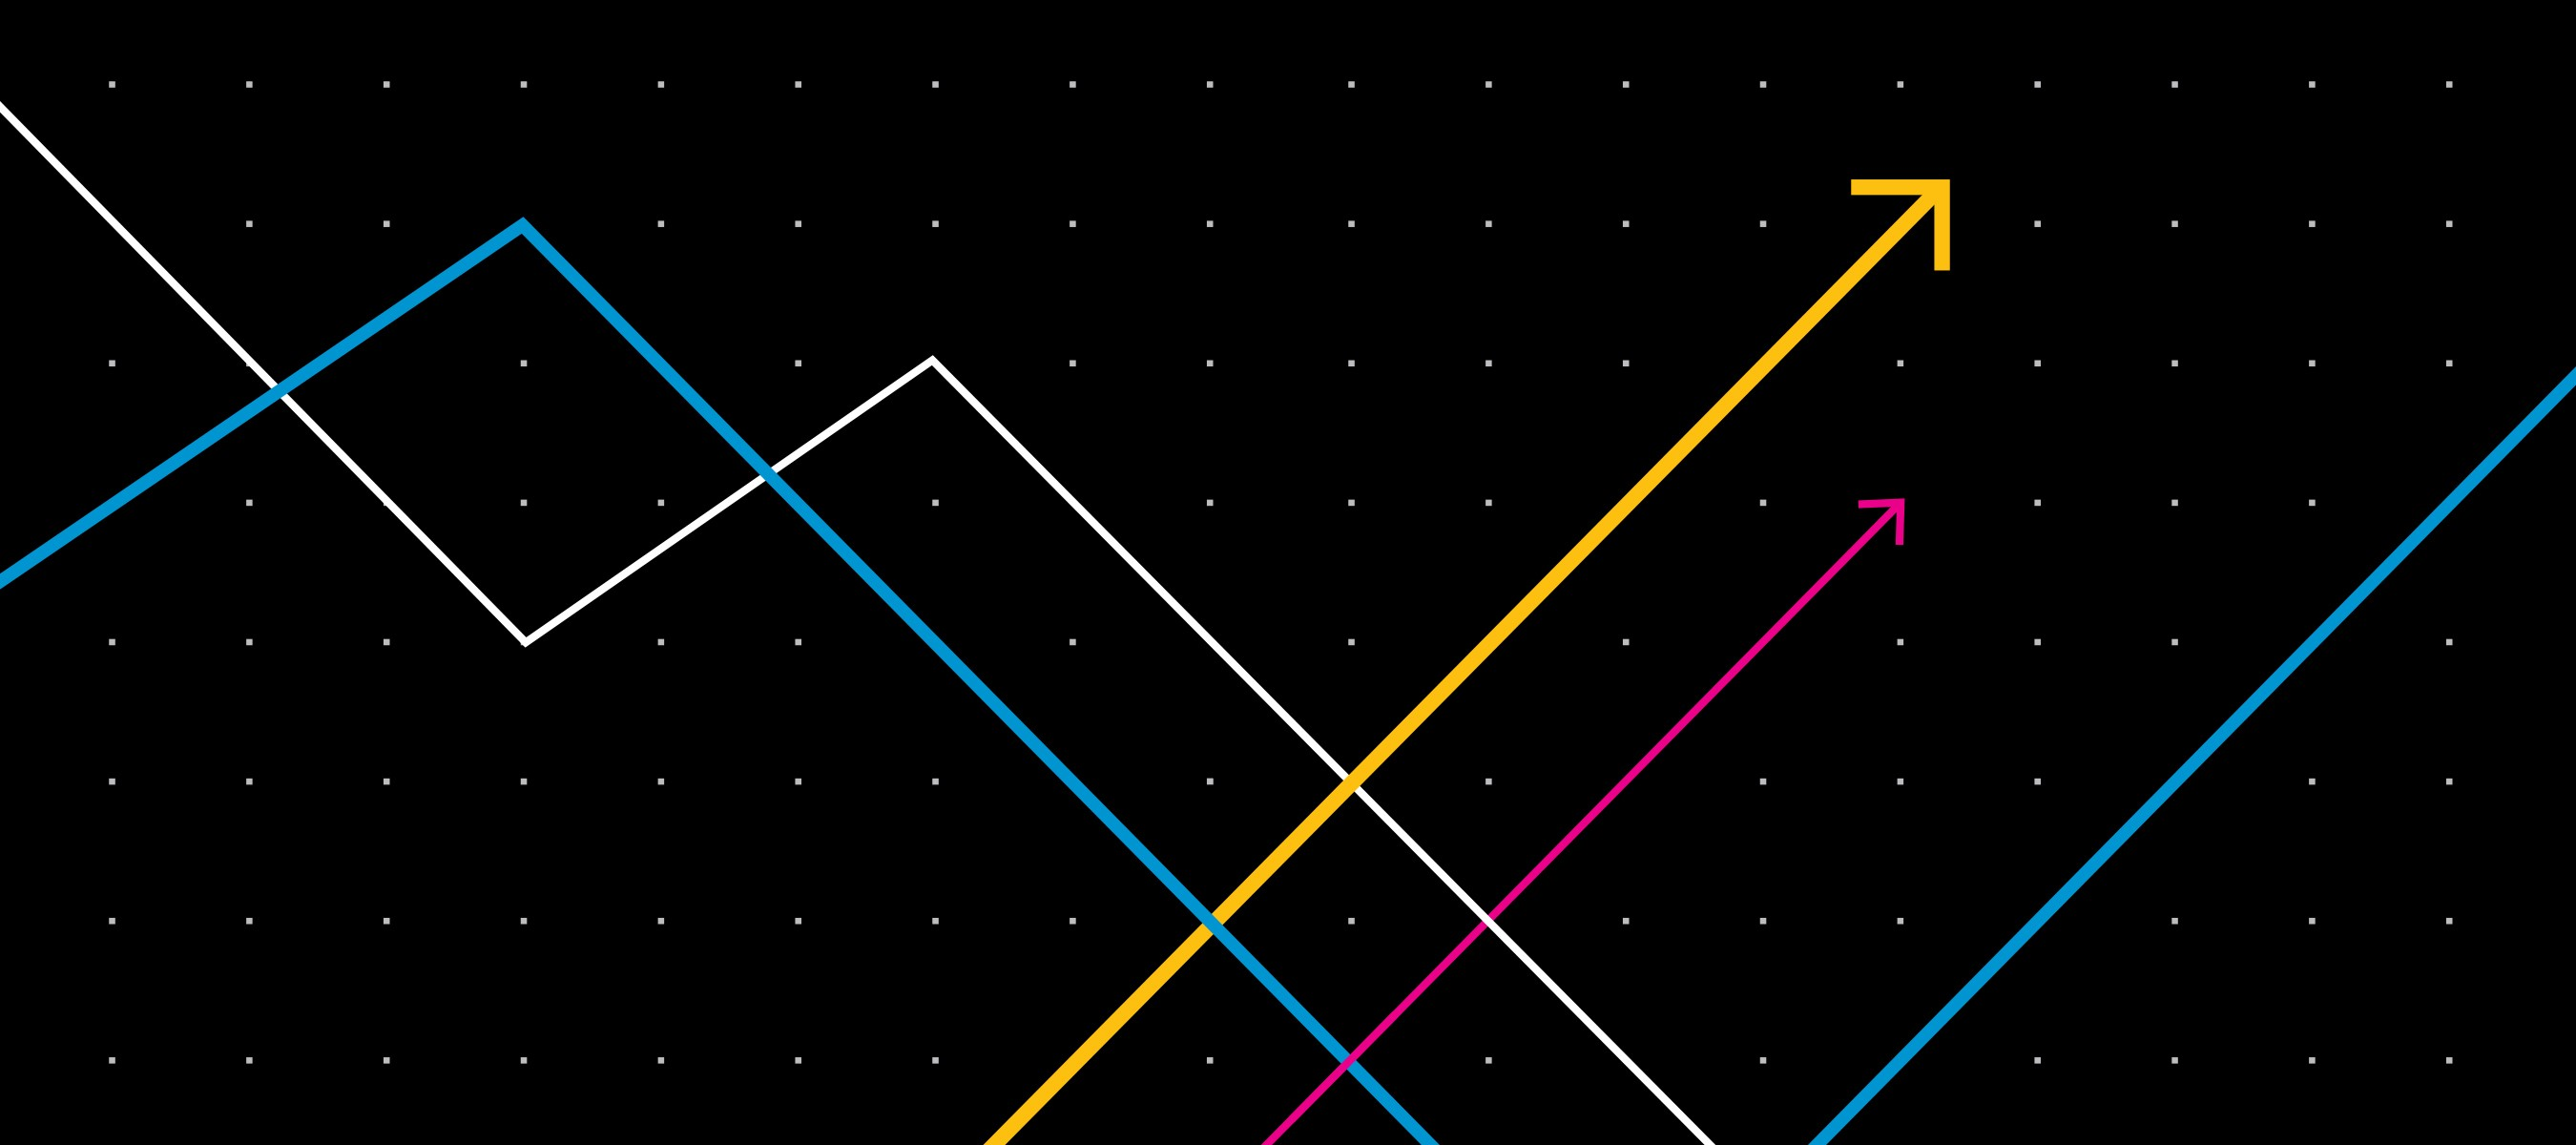
\includegraphics{images/cover.jpg}}
    
    \vspace{0.3in}
    \noindent\textcolor{urban-blue}{\MakeUppercase{\textbf{Research Report}}}
    
    \vspace{0.3in}
    \titlereport{Title Here in Title Case}
    
    \reportsubtitle{Subtitle Here in Title Case}
    
    % Multiple column author names - change the "4" to the number of desired columns
    \begin{multicols}{4}
        \authorfont{Author 1 Name}\\
        \affiliationfont{Author's Affiliation}
        
        \authorfont{Author 2 Name}\\
        \affiliationfont{Author's Affiliation}
        
        \authorfont{Author 3 Name}\\
        \affiliationfont{Author's Affiliation}
        
        \authorfont{Author 4 Name}\\
        \affiliationfont{Author's Affiliation}
    \end{multicols}
    
    \vspace{-0.5cm}
    \authorfont{with Author Name and Author Name}
    
    \datefont{Month and Year}
    \vfill
    \vfill
    \vfill
    
    % Add logo
    \begin{textblock*}{4.5in}[1, 1](5.5in, 10.5in)
        \noindent
\includegraphics[width=4.5in]{images/cover-footer.jpg}
    \end{textblock*}
\end{titlepage}

%%%%%%%%%%%%%%%%%%%%%%%%%%%%%%%%%%%% About Urban %%%%%%%%%%%%%%%%%%%%%%%%%%%%%%%%%%%%%%
\newpage
\thispagestyle{empty} % Removed Page Number
\begin{figure}
    
\includegraphics[width=1.5in]{images/logo.png}
\end{figure}
\vspace*{-0.5in}
\about{About the Urban Institute}\\
\vspace{-5pt}
\boilerplate{The nonprofit Urban Institute is a leading research organization dedicated to developing evidence-based insights that improve people’s lives and strengthen communities. For 50 years, Urban has been the trusted source for rigorous analysis of complex social and economic issues; strategic advice to policymakers, philanthropists, and practitioners; and new, promising ideas that expand opportunities for all. Our work inspires effective decisions that advance fairness and enhance the well-being of people and places.}

\vspace*{\fill}
\begin{singlespace}
    \noindent Copyright ©\tbf{Month Year}. Urban Institute. Permission is granted for reproduction of this file, with attribution to the Urban Institute. Cover image by \tbf{Tim Meko}.
\end{singlespace}

%%%%%%%%%%%%%%%%%%%%%%%%%%%%%%%%%%%% Contents %%%%%%%%%%%%%%%%%%%%%%%%%%%%%%%%%%%%%%
\cleardoublepage
% Set page number to include title page
\setcounter{page}{3}
\begin{singlespace}
    \tableofcontents
\end{singlespace}


%%%%%%%%%%%%%%%%%%%%%%%%%%%%%%%%%%%% Front Matter %%%%%%%%%%%%%%%%%%%%%%%%%%%%%%%%%%%%%%
% Footer Formatting: DO NOT CHANGE -----------------------------------
\fancyfoot{}

\fancyfoot[LE]{\colorbox{urban-footergray}{\makebox(0.2, 0.12)[r]{\fontsize{7.5}{0}\selectfont\bfseries{\MakeUppercase{}\hspace{0.2in}}}}\colorbox{urban-gold}{\makebox(0.2, 0.12)[c]{\fontsize{7.5}{0}\selectfont\bfseries{\MakeUppercase\thepage}}}\colorbox{urban-footergray}{\makebox(5.64, 0.12)[r]{\fontsize{7.5}{0}\selectfont\bfseries{\MakeUppercase{\so{Acknowledgments}}\hspace{0.2in}}}}}

\fancyfoot[RO]{\colorbox{urban-footergray}{\makebox(5.64, 0.12)[l]{\fontsize{7.5}{0}\selectfont\bfseries{\hspace{0.2in}\MakeUppercase{\so{Acknowledgments}}}}}\colorbox{urban-gold}{\makebox(0.2, 0.12)[c]{\fontsize{7.5}{0}\selectfont\bfseries{\MakeUppercase\thepage}}}\colorbox{urban-footergray}{\makebox(0.2, 0.12)[r]{\fontsize{7.5}{0}\selectfont\bfseries{\MakeUppercase{}\hspace{0.2in}}}}}

%%%%%%%%%%%%%%%%%%%%%%%%%%%%%%%%%%%% Acknowledgments %%%%%%%%%%%%%%%%%%%%%%%%%%%%%%%%%%%%
\part{Acknowledgments}

This report was funded by \tbf{[insert your funder name(s) here].} We are grateful to them and to all our funders, who make it possible for Urban to advance its mission. 

The views expressed are those of the \tbf{author/authors} and should not be attributed to the Urban Institute, its trustees, or its funders. Funders do not determine research findings or the insights and recommendations of Urban experts. Further information on the Urban Institute’s funding principles is available at urban.org/fundingprinciples.

\tbf{[Add any other thanks and contract details here. It may be appropriate to also acknowledge your funder’s funder(s). When in doubt, please check with your center director and Contracts.]}

%%%%%%%%%%%%%%%%%%%%%%%%%%%%%%%%%%%% Executive %%%%%%%%%%%%%%%%%%%%%%%%%%%%%%%%%%%%%%%%%
\part{Executive Summary}

\intropara{Body Text style or Chapter Intro Para style here (text shown is in Chapter Intro Para). If you do not have an executive summary, remove this section.}

\section{First-Level Heading in Title Case (Heading 2 style)}

Body Text style for first paragraph under a heading.

Body Text First Indent style for all subsequent paragraphs. \tbf{To add an endnote, use the Insert Endnote function. Endnotes will automatically appear in the Notes section after the appendixes.}\endnote{Endnotes should appear automatically under the Notes heading. If they’re showing up somewhere else, ask your editor or your center’s Word expert for assistance.}

\subsection{Second-Level Heading in Title Case (Heading 3 style)}

Body Text style for first paragraph under a heading.

Body Text First Indent style for all subsequent paragraphs.


\subsubsection{Third-level heading; all caps is built into style (heading 4 style)}

Body Text style for first paragraph under a heading.

Body Text First Indent style for all subsequent paragraphs.

% SPECIAL FOOTER ------
\fancyfoot{}

\fancyfoot[LE]{\colorbox{urban-footergray}{\makebox(0.2, 0.12)[r]{\fontsize{7.5}{0}\selectfont\bfseries{\MakeUppercase{}\hspace{0.2in}}}}\colorbox{urban-gold}{\makebox(0.2, 0.12)[c]{\fontsize{7.5}{0}\selectfont\bfseries{\MakeUppercase\thepage}}}\colorbox{urban-footergray}{\makebox(5.64, 0.12)[r]{\fontsize{7.5}{0}\selectfont\bfseries{\MakeUppercase{Executive Summary}\hspace{0.2in}}}}}

\fancyfoot[RO]{\colorbox{urban-footergray}{\makebox(5.64, 0.12)[l]{\fontsize{7.5}{0}\selectfont\bfseries{\hspace{0.2in}\MakeUppercase{Executive Summary}}}}\colorbox{urban-gold}{\makebox(0.2, 0.12)[c]{\fontsize{7.5}{0}\selectfont\bfseries{\MakeUppercase\thepage}}}\colorbox{urban-footergray}{\makebox(0.2, 0.12)[r]{\fontsize{7.5}{0}\selectfont\bfseries{\MakeUppercase{}\hspace{0.2in}}}}}

%%%%%%%%%%%%%%%%%%%%%%%%%%%%%%%%%%%% Main Text %%%%%%%%%%%%%%%%%%%%%%%%%%%%%%%%%%%%%%
% Setting the page numbers to be arabic
\pagenumbering{arabic}

\part{Report Title Here in Title Case (Heading 1 style)}

Body Text style for first paragraph.

Body Text First Indent style for subsequent paragraphs. \textcolor{red}{To add an endnote, use the Insert Endnote function. Endnotes will automatically appear in the Notes section after the appendixes.}\endnote{Endnotes inserted in the executive summary, main report, and appendixes will all display here if section breaks are used correctly.} 

\section{First-Level Heading in Title Case (Heading 2 style)}

Body Text style for first paragraph under a heading.

Body Text First Indent style for all subsequent paragraphs.
\begin{itemize}
    \item Bulleted List style for bulleted lists.
    \item Another bullet using Bulleted List style.
    \begin{itemize}
        \item Bulleted List 2 style for second-level bulleted items under a numbered or bulleted list item.
        \item Another item using Bulleted List 2 style.
    \end{itemize}
    \item Another bullet using Bulleted List style.\\
    Indented Text style for ordinary paragraphs under a numbered or bulleted list item.
\end{itemize}

\noindent Body Text First Indent style for all subsequent paragraphs.

\begin{enumerate}
    \item Numbered List style for numbered lists
    \begin{enumerate}
        \item Numbered List 2 style for second-level lettered items under a numbered or bulleted list item.
        \item Another paragraph using Numbered List 2 style.
    \end{enumerate}
    \item Another item using Numbered List style.\\
    Indented Text style for ordinary paragraphs under a numbered or bulleted list item.
\end{enumerate}

\noindent Body Text First Indent style for all subsequent paragraphs.

\subsection{Second-Level Heading in Title Case (Heading 3 style)}

\indent Body Text style for first paragraph under a heading.

\subsubsection{Third-level heading; all caps is built into style (heading 4 style)}

Body Text style for first paragraph under a heading.

\fourthsub{Fourth-level headings are run into the text.} Select the first clause or sentence of your paragraph, then apply the Heading 5 (D) style. 

Pull Quote style for pull quotes.

---Pull quote attribution in sentence case

Body Text First Indent style for all subsequent paragraphs.

\block{Block Text style for longer (100+ words) quotes and excerpts.}

\newpage
\part{Reference Styles for Urban Products}

\section{Blog posts (cite in notes, not reference list)}

\section{Policy debates (cite in notes, not reference list)}

\subsection{The entire debate:}

\subsection{One post in the debate:}

\cite{Ful83}

%%%%%%%%%%%%%%%%%%%%%%%%%%%%%%%%%%%% Back Matter %%%%%%%%%%%%%%%%%%%%%%%%%%%%%%%%%%%%%%
%%%%%%%%%%%%%%%%%%%%%%%%%%%%%%%%%%%% Appendix %%%%%%%%%%%%%%%%%%%%%%%%%%%%%%%%%%%%%%%%%%%
\part{Appendix Letter. Appendix Title in Title Case}

Use the same text styles you used in the main report.

% SPECIAL FOOTER ------
\fancyfoot{}

\fancyfoot[LE]{\colorbox{urban-footergray}{\makebox(0.2, 0.12)[r]{\fontsize{7.5}{0}\selectfont\bfseries{\MakeUppercase{}\hspace{0.2in}}}}\colorbox{urban-gold}{\makebox(0.2, 0.12)[c]{\fontsize{7.5}{0}\selectfont\bfseries{\MakeUppercase\thepage}}}\colorbox{urban-footergray}{\makebox(5.64, 0.12)[r]{\fontsize{7.5}{0}\selectfont\bfseries{\MakeUppercase{Appendix}\hspace{0.2in}}}}}

\fancyfoot[RO]{\colorbox{urban-footergray}{\makebox(5.64, 0.12)[l]{\fontsize{7.5}{0}\selectfont\bfseries{\hspace{0.2in}\MakeUppercase{Appendix}}}}\colorbox{urban-gold}{\makebox(0.2, 0.12)[c]{\fontsize{7.5}{0}\selectfont\bfseries{\MakeUppercase\thepage}}}\colorbox{urban-footergray}{\makebox(0.2, 0.12)[r]{\fontsize{7.5}{0}\selectfont\bfseries{\MakeUppercase{}\hspace{0.2in}}}}}

%%%%%%%%%%%%%%%%%%%%%%%%%%%%%%%%%%%% Notes %%%%%%%%%%%%%%%%%%%%%%%%%%%%%%%%%%%%%%
\theendnotes


%%%%%%%%%%%%%%%%%%%%%%%%%%%%%%%%%%%% References %%%%%%%%%%%%%%%%%%%%%%%%%%%%%%%%%%%%%%
\bibliographystyle{chicago}
{
    \fontsize{9}{9}%
    \selectfont%
    \bibliography{references}
}

%%%%%%%%%%%%%%%%%%%%%%%%%%%%%%%%%%%% About Author %%%%%%%%%%%%%%%%%%%%%%%%%%%%%%%%%%%%%%
\part{About the Authors}

\textbf{Author Name in Bold} but the rest of the text lightface. Use Author Bios--First style for the introductory paragraph of each bio. You can paste your bio from your author page on the Urban website (and condense it if needed) here.\\
If your bio is more than one paragraph long, use Author Bios--Additional for any subsequent paragraphs. This style suppresses spacing between paragraphs.\\
Author bios no longer include photos.

\noindent\textbf{Author Name in Bold} but the rest of the text lightface. Use Author Bios--First style for the introductory paragraph of each bio. You can paste your bio from your author page on the Urban website (and condense it if needed) here.\\
If your bio is more than one paragraph long, use Author Bios--Additional for any subsequent paragraphs. This style suppresses spacing between paragraphs.\\
Author bios no longer include photos.


% SPECIAL FOOTER ------
\fancyfoot{}

\fancyfoot[LE]{\colorbox{urban-footergray}{\makebox(0.2, 0.12)[r]{\fontsize{7.5}{0}\selectfont\bfseries{\MakeUppercase{}\hspace{0.2in}}}}\colorbox{urban-gold}{\makebox(0.2, 0.12)[c]{\fontsize{7.5}{0}\selectfont\bfseries{\MakeUppercase\thepage}}}\colorbox{urban-footergray}{\makebox(5.64, 0.12)[r]{\fontsize{7.5}{0}\selectfont\bfseries{\MakeUppercase{About the Authors}\hspace{0.2in}}}}}

\fancyfoot[RO]{\colorbox{urban-footergray}{\makebox(5.64, 0.12)[l]{\fontsize{7.5}{0}\selectfont\bfseries{\hspace{0.2in}\MakeUppercase{About the Authors}}}}\colorbox{urban-gold}{\makebox(0.2, 0.12)[c]{\fontsize{7.5}{0}\selectfont\bfseries{\MakeUppercase\thepage}}}\colorbox{urban-footergray}{\makebox(0.2, 0.12)[r]{\fontsize{7.5}{0}\selectfont\bfseries{\MakeUppercase{}\hspace{0.2in}}}}}

%%%%%%%%%%%%%%%%%%%%%%%%%%%%%%%%%%%% Statement of Independence %%%%%%%%%%%%%%%%%%%%%%%%%%
\addcontentsline{toc}{part}{Statement of Independence}
\thispagestyle{empty} 

\about{Statement of Independence}
\vspace{-5pt}
\boilerplate{The nonprofit Urban Institute is a leading research organization dedicated to developing evidence-based insights that improve people’s lives and strengthen communities. For 50 years, Urban has been the trusted source for rigorous analysis of complex social and economic issues; strategic advice to policymakers, philanthropists, and practitioners; and new, promising ideas that expand opportunities for all. Our work inspires effective decisions that advance fairness and enhance the well-being of people and places.}

%%%%%%%%%%%%%%%%%%%%%%%%%%%%%%%%%%%% Back Cover %%%%%%%%%%%%%%%%%%%%%%%%%%%%%%%%%%%%%%
\newpage
\thispagestyle{empty}

\begin{textblock*}{8.5in}[1, 1](8.5in, 11in)
    \noindent
\includegraphics[width=\paperwidth,height=\paperheight]{images/back.pdf}
\end{textblock*}

\end{document}
